\section{Analisi multivariata e Machine Learning}
\label{analisi multivariata e ML}

	Quando si parla di analisi dati ci si può essenzialmente ricondurre a tre macro-categorie di operazioni:

\begin{enumerate}
	\item CLASSIFICAZIONE \\
	Questa tipologia è probabilmente la principale quando si ha a che fare con la fisica delle alte energie e consiste nell'associare un evento/oggetto  ad una categoria. Nel caso specifico di questa trattazione l'obiettivo sarà esattamente quello di classificare gli eventi/oggetti nelle due categorie di background e segnale.

	\item STIMA DI PARAMETRI \\
	In questa tipologia ricadono tutti quei processi attraverso i quali si estraggono dei parametri (ad esempio la massa di una tipologia di particelle) attraverso un fitting del modello teorico con i dati sperimentali;
	
	\item STIMA DI FUNZIONI \\
	Si ricava una funzione continua di una o più variabili a partire dai dati sperimentali.
\end{enumerate}

Questa trattazione si concentrerà essenzialmente sulle possibili metodologie di classificazione, proprio perché l'obiettivo è il discernimento fra segnale e background alla ricerca di nuova fisica. \\
Nelle prime righe di questo capitolo è stato introdotto il termine $\textit{evento}$ o $\textit{oggetto}$, senza meglio specificare come questo fosse collegato ai dati. Un evento può essere pensato come una collezione di dati e quindi lo si può rappresentare come un vettore in uno spazio n-dimensionale: 
\begin{equation}
\textbf{x} = (x_{1},...,x_{n})
\end{equation}
In realtà l'utilizzo del termine vettore è improprio ogni qual volta si abbia a che fare con componenti (i dati) disomogenee tra loro, tuttavia lo si continuerà ad utilizzare per una questione di comodità tenendo a mente questa specifica. Nelle pagine successive con i termini evento, oggetto, vettore di input e pattern ci si riferirà sempre alla stessa entità appena introdotta. \\ 
Una volta presentate queste notazioni è possibile focalizzarsi sui diversi approcci che possono essere seguiti per tentare di separare il segnale dal background quando si ha a disposizione una grande mole di dati. Nelle righe che seguono verranno presentati tre diverse metodologie, dalla più semplice ed inefficiente a quella più complessa e raffinata:
\begin{enumerate}
	\item Sistema di tagli sulle variabili, ovvero il metodo più semplice ma anche meno efficiente. Non può essere considerato un metodo multi-variato per le ragioni che si vedranno a breve;
	\item Analisi multi-variata e, nello specifico, l'analisi discriminante lineare;
	\item Machine Learning, dove entra in gioco il concetto di apprendimento automatico e quindi si dispone di tecniche che permettono all'algoritmo di imparare in maniera autonoma direttamente dai dati che gli vengono forniti.
\end{enumerate}

\newpage

\subsection{Sistema di tagli}
\label{sistema di tagli}
Un primissimo semplice approccio prevede di adoperare dei tagli sulle varie componenti dei pattern, in modo da ricavare un ipercubo nello spazio n-dimensionale dei pattern stessi. Per capire meglio questa metodologia si consideri un caso semplificato nel quale lo spazio in questione è bi-dimensionale e quindi i vettori di input sono del tipo $\textbf{x} = (x_1,x_2)$; per raggiungere l'obiettivo di separazione bisognerà dunque applicare due tagli, uno sulla variabile $x_1$ ed uno su $x_2$, stabilendo un punto $\textbf{P} = (P_1,P_2)$ come riportato in figura ~\ref{fig:grid_example}.

\begin{figure}[h!]
	\centering
	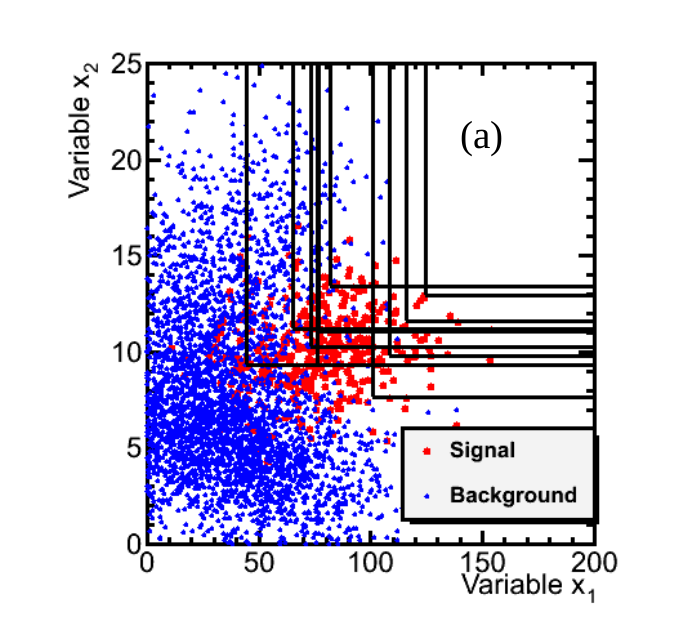
\includegraphics[width=0.85\textwidth]{figs/Grid_example.png}
	\caption{risultato grafico di un processo di taglio sulle due variabili $x_1$ e $x_2$ per la separazione del segnale dal background (\cite{Metodi_multivariati}).}
	\label{fig:grid_example}
\end{figure}

Chiaramente la scelta del punto $\textbf{P}$ non è casuale e deve essere ottimizzata; un metodo per raggiungere tale obiettivo è il Random Grid Search (RGS) che verrà presentato nella sezione ~\ref{iperparametri e grid search}. \\
In questo caso, nonostante si abbia a che fare con pattern multi-dimensionali, non è possibile parlare di approccio multivariato, perché i tagli sulle singole dimensioni sono indipendenti fra loro; ecco che si capisce che il prezzo da pagare per la grande semplicità di questo metodo è la sua scarsa efficienza, infatti i tagli che possono essere ottenuti sono paralleli agli assi e ciò è estremamente limitante.

\newpage

\subsection{Processi multivariati e analisi discriminante lineare}
\label{metodi lineari e discriminante di Fisher}

Per poter fare un passo in avanti nella trattazione bisogna considerare la possibilità che le varie componenti dei vettori evento siano tra loro correlate o, più in generale, bisogna considerare tali pattern nella loro totalità, ovvero senza focalizzarsi sulle singole componenti in maniera separata (come è stato fatto con il sistema di tagli).  Per la ragione appena presentata è necessario considerare i processi multi-variati.	Dato che le componenti dei pattern possono essere tra loro correlate è possibile ridurre la dimensionalità dello spazio n-dimensionale da n a d (con d < n). Verrà posto un focus particolare sul problema della dimensionalità degli input della sezione ~\ref{curse_dim}, che servirà da trampolino di lancio per affrontare un metodo particolare del ML, il Variational Autoencoders. \\
Come detto nella sezione precedente, i sistemi di tagli possono essere utilizzati per la separazione del segnale dal fondo ma hanno dei limiti piuttosto considerevoli che sono già stati illustrati. L'analisi discriminante è un metodo che permette di raggiungere lo stesso obiettivo di separazione, ma in modo più efficiente. \\
L'analisi discriminante si definisce lineare quando la funzione classificatrice è, appunto, lineare. \\
Si immagini di avere a disposizione un determinato set di eventi in input $\textbf{x}_\textbf{i}$, ciascuno caratterizzato da un numero n di variabili (spazio n-dimensionale) e di volerli ripartire fra segnale e background.\\
Si definisce la funzione discriminante lineare nel seguente modo:
\begin{equation}
D(x_1 , x_2 , ... , x_n) = c_0 + c_1x_1 + ... +c_nx_n = c_0 + \sum_{i=0}^{n} c_ix_i 
\end{equation}
quindi come una combinazione lineare delle componenti del vettore che rappresenta l'evento; il valore assunto dalla funzione per ogni singolo evento ne permette la separazione nelle due classi (nel presente caso segnale e background), utilizzando un valore di riferimento $D_0$. \\
A questo punto l'obiettivo è quello di massimizzare la distanza fra le due classi, ovvero rendere massima la differenza dei valori assunti dalla funzione $D(\textbf{x})$ fra gli eventi appartenenti al background e quelli relativi al segnale. \\
Un esempio di questo approccio è il metodo proposto da Fisher: si consideri un campione di eventi appartenenti al segnale e se ne definisca la media $\bm\mu_\textbf{s}$ e la deviazione standard $\sigma_s$ ed un campione appartenente al background, definendo anche qui la media $\bm\mu_\textbf{f}$ e la deviazione standard $\sigma_f$. A questo punto la migliore configurazione dei parametri è quella che massimizza la seguente funzione: 
\begin{equation}
F(\textbf{c}) = \frac{(\bm\mu_\textbf{s} - \bm\mu_\textbf{f})^2}{\sigma_s^2 + \sigma_f^2}
\end{equation} 
Il pregio di un'analisi di questo tipo è quello di non doversi necessariamente limitare a dei tagli paralleli agli assi. 

\newpage

\subsection{Machine Learning}
\label{ML}
Proseguendo nel percorso intrapreso per l'ottimizzazione nella separazione del segnale dal background, si è giunti a trattare uno degli argomenti centrali di questo lavoro, il Machine Learning (ML).\\
Perché è utile il ML per l'obiettivo che è stato prefissato? La risposta sta nel fato che un algoritmo di ML è in grado di apprendere in maniera semi-autonoma a partire dai dati che gli vengono presentati e quindi sarà l'algoritmo stesso a stabilire quale sia la migliore forma con la quale delimitare lo spazio n-dimensionale dei vettori di input nelle due zone relative al segnale ed al background. \\
Tuttavia, prima di presentare il metodo di ML che verrà utilizzato per raggiungere l'obiettivo di classificazione segnale-background, verrà svolta un'ampia panoramica sul ML e sulle metodologie più comuni. \\
L'approccio classico all'analisi dei dati prevede la disponibilità di un modello matematico, che dipende da una serie di parametri incogniti. Questi parametri vengono ricavati a partire dai dati sperimentali attraverso processi che possono essere sia analitici che numerici. \\
Quando si parla di machine learning la prospettiva viene ribaltata, perché il modello matematico non è noto a priori. \\
Bisogna distinguere tre macro-tipologie di approccio all'analisi dati nel machine learning:
\begin{itemize}
	\item APPRENDIMENTO SUPERVISIONATO \\
	In questa tipologia di apprendimento vengono presentati al computer degli input di esempio ed i relativi output desiderati, con lo scopo di apprendere una relazione generale che lega gli input con gli output; in questo caso si utilizza il così detto "training data set", mentre per testare il modello ottenuto si considera il "test data set" dove non vengono forniti al computer gli output. L'apprendimento supervisionato verrà trattato in maniera più approfondita nel prossimo paragrafo.
	\item APPRENDIMENTO NON SUPERVISIONATO \\
	In questo caso non vengono forniti al computer gli output attesi fin dalle prime fasi di apprendimento del modello e quindi lo scopo è quello di scoprire una qualche struttura fra i dati di input.%\comment{fare riferimento al variational autoencoder: La parte implementativa di questa tesi si basa sull'utilizzo di un algoritmo unsupervised meglio noto come variational autoencoder.
	Come si vedrà, questo modello viene addestrato per identificare le caratteristiche peculiari degli eventi fisici di background in modo da contrapporli successivamente a quelle relative ad eventi di segnale.\\
	Verrà posta attenzione su un particolare metodo di apprendimento non supervisionato, il Variational Autoencoder (VAEs), del quale verrà svolta una trattazione teorica approfondita ed una applicazione al campo della fisica delle particelle
	\item APPRENDIMENTO PER RINFORZO \\
	Il Reinforcement Learning è basato sul concetto di ricompensa, ovvero si permette all'algoritmo di esplorare un così detto ambiente e, in base all'azione compiuta, gli si fornisce un feedback positivo, negativo o indifferente. Un esempio classico prevede di voler addestrare un algoritmo per un particolare gioco: si farà in modo di fargli compiere una serie di partite in maniera iterativa e gli si assegnerà una ricompensa in caso di vittoria o un malus in caso di sconfitta. \\ 
\end{itemize}

\newpage

Una ulteriore distinzione che è necessario fare è fra algoritmi di classificazione, regressione e clustering:
\begin{itemize}
	\item CLASSIFICAZIONE \\
	Gli algoritmi di classificazione sono caratterizzati da un output discreto, cioè una serie di classi alle quali l'input può appartenere.Questa tipologia di meccanismo viene in genere portata avanti tramite metodi di apprendimento supervisionato. Un esempio di algoritmo di classificazione è quello che permette di distinguere se un particolare oggetto è presente o meno in un'immagine.
	\item REGRESSIONE \\
	La regressione è simile alla classificazione con la differenza che, in questo caso, l'output è continuo. Anche gli algoritmi di regressione sono adatti ad essere trattati con metodologie di apprendimento supervisionato.
	\item CLUSTERING \\
	Nel clustering l'obiettivo è sempre quello di dividere gli input in delle classi, tuttavia in questo caso tali classi non sono stabilite a priori. La natura di algoritmi di questo tipo li rende adatti ad essere trattati tramite metodi di apprendimento non supervisionato.
\end{itemize}

